\chapter{Fundamentos teóricos}\label{ch:fundamento-teorico}

Este capítulo incluye un resumen de los enfoques, teorías y conceptos en los cuales se fundamenta el trabajo del proyecto de grado. Se basa, principalmente, en la exposición de otros trabajos sobre los temas estudiados, buscando cierto nivel de auto-contención en el documento. En otras palabras, el objetivo de este capítulo es guiar al lector en la interpretación de trabajos que se han ocupado previamente de la cuestión central de esta tesis, incluyen conocimiento de base para este trabajo u ofrecen herramientas analíticas o interpretativas para los estudios realizados. 
Específicamente, en este capítulo se incluyen conceptos introductorios sobre matrices dispersas, en especial los formatos más comunes para almacenarlas, así como el uso de hardware para computación de alta performance (HPC por su sigla en inglés --High Performance Computing--) con foco en el uso de los procesadores gráficos o simplemente GPUs.


\section{Matrices dispersas} \label{sparse-intro}

Para iniciar los conceptos, primero se presenta una definición formal de matriz. Una matriz es un arreglo bidimensional de números dispuestos en filas y columnas, donde dichos números frecuentemente representan los coeficientes de un sistema lineal. En cuanto a la notación, típicamente las matrices se llaman con letras mayúsculas $(A)$ y quedan definidas por sus dimensiones, es decir, la cantidad de filas y columnas que dispone. Las entradas del arreglo se denominan coeficientes, comúnmente identificados con letra minúscula y dos subíndices que indican fila y columna respectivamente $(a_{ij})$. Ver Figura~\ref{fig:A-matrix} por un resumen gráfico.


El concepto de matriz dispersa no cuenta con una definición específica. En forma conceptual, se puede considerar como aquellas matrices ``grandes'' que incluyen ``una porción importante'' de coeficientes con valor nulo. Es claro que ``grandes'' y ``una porción importante'' son términos ambiguos para referirse a las características de las matrices ya que dependen del contexto de aplicación. Por ejemplo, una matriz en los años 60s, podía considerarse grande y en la actualidad ser una matriz pequeña. 
% Alineado con lo descrito anteriormente, se incluye la definición y un panorama general de las matrices dispersas expresado por Tim Davis :%\cite{TimDavis}.
Según Tim Davis~\cite{TimDavis} las matrices dispersas que surgen de los problemas del mundo real, tanto en ciencia, ingeniería, matemática y otras áreas, tienden a ser dispersas. Los algoritmos que trabajan con dichas matrices, se encuentran en la intersección de la teoría de grafos y el álgebra lineal numérica. Un grafo puede representar las conexiones entre variables en el modelo matemático, como el voltaje a través de un componente de un circuito, un enlace de una página web a otra, las fuerzas físicas entre dos puntos en una estructura mecánica, etc. El álgebra lineal numérica surge porque estas matrices representan sistemas de ecuaciones cuya solución nos dice algo sobre cómo se comporta el problema del mundo real. Por ejemplo, el algoritmo \textit{page rank}~\cite{pagerank} de Google, requiere el cálculo de un vector propio para una matriz con tantas filas y columnas como páginas en la Web. %Haciendo hincapié en la gran cantidad de problemas para los que aplican este tipo de estudios.

% \textit{``The large matrices that arise in real-world problems in science, engineering, and mathematics tend to be mostly zero, or sparse.  Sparse matrix algorithms lie in the intersection of graph theory and numerical linear algebra.  A graph represents the connections between variables in the mathematical model, such as the voltage across a circuit component, a link from one web page to another, the physical forces between two points in a mechanical structure, and so on, depending on the problem at hand.  The numerical linear algebra arises because these matrices represent systems of equations whose solution tells us something about how the real-world problem behaves.  Google’s page rank algorithm, for example, requires the computation of an eigenvector for a matrix with as many rows and columns as there are pages on the web''}. Extraído de~\cite{davis-sparse-def}.


Otro aspecto relacionado con las matrices dispersas es el almacenamiento. Para hablar de matrices dispersas es necesario que se utilice un formato de almacenamiento que saque partido (al menos que lo intente) de los coeficientes con valor 0\footnote{En campos de aplicación específicos podría ser dispersa con respecto a otro valor. En este caso, se usa 0 como valor nulo.}. Es decir, si se tiene una matriz grande y con muchos coeficientes nulos, pero está almacenada en el formato tradicional, no es posible sacar partido de esta propiedad y, en la práctica, su tratamiento será idéntico al de una matriz densa.

\begin{figure}
    \centering
     $$ A = 
    \begin{pmatrix} 
    a_{11} & a_{12} & \dots & a_{1n} \\
    a_{21} & a_{22} & \dots & a_{2n} \\
    \vdots & \vdots & \ddots  & \vdots\\
    a_{m1} & a_{m2} & \dots & a_{mn} \\
    \end{pmatrix}
    \quad
    $$
    \caption{Matriz de tamaño $m\times n$.}
    \label{fig:A-matrix}
\end{figure}



% En este proyecto serán abordadas principalmente matrices, cuadradas, es decir de tamaño $n\times n$

En el contexto de este proyecto, para la definición de matriz dispersa, se pondrá foco en el uso de alguna estrategia de almacenamiento que saque partido de la proporción de coeficientes no nulos. Para esto, se presenta el concepto de densidad de una matriz dispersa~\cite{density-matlab}, magnitud que permite de cierto modo cuantificar cuán dispersa es una matriz. Esta se define como $\rho = \frac{\nnz}{m \times n}$, donde $\nnz$ es la cantidad de elementos no nulos de la matriz, siendo $m$ y $n$ la cantidad de filas y columnas respectivamente. Se considera dispersas, en general, a aquellas matrices que presentan valores de densidad por debajo del 1\%. Sobre las dimensiones de la matriz no se pondrán restricciones, pero recordando que, en los dispositivos actuales, las matrices que al menos tengan centenas o miles  de filas/columnas son las que presentan real interés. 

En este contexto, es claro que dichas matrices se pueden almacenar en memoria de diferentes formas, omitiendo al menos la gran mayoría de los elementos nulos. Como ejemplo, notar que, utilizando la forma convencional de almacenamiento (matriz densa), una matriz de $10^4 \times 10^5$ elementos utilizando aritmética de punto (o coma) flotante de doble precisión (\texttt{64 bits}, i.e. \texttt{8 Bytes}) para los coeficientes, implica el uso de un total de $10^4 \times 10^5 \times 8$ \texttt{Bytes} $ = 8\times 10^9$ \texttt{Bytes} $ = 8$ \texttt{GBytes}. En caso de tener una densidad del $1\%$, es decir $10^7$ coeficientes no nulos y poder almacenar únicamente estos coeficientes, implicaría un almacenamiento de $0.08$ \texttt{GBytes}. Este razonamiento permite observar los posibles ahorros en memoria, aunque es claro que se necesitará información extra para indicar al menos las posiciones de los coeficientes.

% (Quizas un ejemplo mas visual? tomando $n = 10^5$, si se quisiera almacenar la matriz de tamaño $n \times n$ en un arreglo bidimensional, guardando todos los datos en doble precisión, se necesitarían $10^5 \times 10^5 \times 8$ \texttt{Bytes} $= 8 \times 10^{10}$ \texttt{Bytes} $= 80$ \texttt{GBytes}. Si la matriz, por ejemplo, tuviese una estructura tridiagonal, esta puede fácilmente, ignorando las entradas nulas, ser almacenada en tres arreglos de  $10^5$ entradas, dando un total aproximado de $3 \times 8 \times 10^5$ \texttt{Bytes} = $2.4$ \texttt{MBytes})



% El hecho de utilizar un formato de almacenamiento para las matrices dispersas va mas allá de ahorrar en almacenamiento, sino también, tiene como segundo objetivo agilizar y/o ahorrar en lo posible, cantidad de cálculos a la hora de trabajar con dichas matrices.

Si bien se desprende de los párrafos anteriores que, se pueden lograr grandes ahorros en memoria con el simple hecho de guardar solamente los elementos no nulos y sus correspondientes coordenadas o índices que permitan identificar cada una de estas entradas dentro de la matriz, esto no garantiza una representación óptima (o eficiente) a la hora de operar con dicha matriz. Interesa, entonces, encontrar cierto balance en las características del formato de almacenamiento, de modo de poder optimizar tanto requerimientos de memoria como de cómputo.

% Los formatos de almacenamiento se pueden dividir en dos grandes grupos: los estáticos y los dinámicos, de los cuales se desprenden nociones de en qué casos corresponde utilizar uno u otro. Esta clasificación se aborda con algo más de profundidad en la Sección~\ref{formatos}. 

Como se mencionó antes, las características de las matrices pueden ser muy variadas dependiendo de los problemas que éstas representan o intentan resolver, dando lugar a estructuras particulares que algunos formatos intentan explotar. Muy a grandes rasgos, según las propiedades o características de las matrices, determinadas por la disposición de los elementos no nulos (concepto denominado patrón de la matriz~\cite{Belgin2010}), se las puede clasificar en las siguientes categorías:
% alpha
% Conceptos como: ancho de banda (bandwidth), matriz traspuesta

% \begin{itemize}
%     \item DEF Matriz traspuesta\\
%      Sea $A = ((a_{ij}))$ una matriz $n\times m$, definimos la matriz traspuesta de $A$ como la matriz $m \times n$ $A^t = ((a^t_{ij}))$, donde $a^t_{ij} = a_{ji}$.
%     \item DEF Ancho de banda (bandwidth) ..

% \end{itemize}
%  Definidos los conceptos necesarios, a continuación se describen algunas categorías determinadas por las características de las matrices:

\begin{itemize}
    \item  \textbf{de banda:}
    se dice que una matriz es de banda cuando tanto el ancho de banda (la mayor distancia de un elemento no nulo a la diagonal) inferior como el superior son razonablemente ``pequeños''.
    Expresado matemáticamente, una matriz $A$ de tamaño $n \times n$, es una matriz de banda si todos sus elementos no nulos están comprendidos dentro de un rango o zona entorno a la diagonal principal. % determinado por los valores $k_1$ y $k_2$.
    Entonces $a_{ij} \neq 0$ si $i - j < k_1$ o $j - i < k_2$  % o lo que es lo mismo     $a_{ij} = 0$ si $j < i - k_1$ o $j > i + k_2;$ $k_1,k_2 \geq 0$ (que los elementos fuera del rango tomen el valor 0).
    , donde $k_1$ y $k_2$ corresponden a los semi-anchos izquierdo (inferior) y derecho (superior) respectivamente. 
    En la literatura, algunos autores definen el ancho de banda de una matriz en base a los semi-anchos, obteniendo:
    \begin{equation*}\label{bandwidth}
        \beta(A) = max\{k_1, k_2\}.
    \end{equation*}
    Otros, de forma equivalente, directamente definen el ancho de banda en base a los índices de los coeficientes no nulos. Por ejemplo, George et  al. \cite{comp-sol-of-sparse-linear-systems} definen el ancho de banda de una matriz $A$ de la siguiente manera:
    \begin{equation*}\label{bandwidth}
        \beta(A) = max\{|i -  j|\ |\ a_{ij} \neq 0 \}.
    \end{equation*}
    
    También es importante considerar el concepto de \textit{profile}. El profile de una matriz $A$, simétrica, está definido como: $profile(A) = \sum_{i = 1}^{n} \beta_i (A)$, donde $\beta_i (A)$ es el ancho de banda en la fila $i$-ésima de la matriz $A$. Es decir, la distancia máxima de un valor no nulo de la fila $i$ a la diagonal. 

    %\item  \textbf{diagonales}
    \item \textbf{diagonal:} un caso extremo de matriz de banda, son las matrices diagonales, donde la banda está compuesta por una única diagonal.
    \item  \textbf{simétricas} (o \textbf{hermíticas} en el caso complejo):
    una matriz $A$ es simétrica sí y solo sí $A = A^t$ o $a_{i j} = a_{ji}$, para todo valor válido de $i$ y $j$, es decir, que sean menores o iguales a la cantidad de filas y columnas respectivamente. En el caso complejo, $a_{ij} = \overline{a_{ji}}$. Un ejemplo común de donde aparecen estas matrices son los grafos bidireccionales o no dirigidos.
    \item  \textbf{de bloques:}
    una matriz de bloques, es una matriz que se puede interpretar como la composición de varias sub-matrices o bloques cuadrados de dimensiones $n_b$. En particular, para matrices dispersas, la división de estos bloques se realiza de forma que estos contengan todos los elementos no nulos, dejando por fuera la mayor cantidad de elementos nulos, ver apartados \ref{bccs} y \ref{bcrs}.
    \item \textbf{cantidad constante de elementos por fila/columna:} son las matrices que presentan la misma cantidad de elementos no nulos en todas las filas (o columnas). Una clase importante de problemas ofrecen esta característica y los formatos asociados también son particulares.
    
\end{itemize}


\section{Formatos de almacenamiento}\label{formatos}

A la hora de almacenar este tipo de matrices, como se menciona en la Sección~\ref{sparse-intro} existen varias estrategias, clasificadas principalmente en dos grandes grupos, estáticas y dinámicas. Parece importante mencionar, y de forma breve explicar, como funcionan los formatos clásicos  para almacenar matrices dispersas.

\begin{figure}
\begin{center}
\begin{eqnarray*}
A = \left(
\begin{array}{ccccccc} 
1 & 2 & 0 & 0 & 3 & 4 & 0\\
0 & 5 & 0 & 6 & 0 & 0 & 0\\
0 & 7 & 8 & 9 & 0 & 0 & 0\\
1 & 0 & 0 & 2 & 0 & 0 & 0\\
0 & 3 & 0 & 0 & 4 & 5 & 0\\
0 & 0 & 6 & 0 & 7 & 8 & 0\\
0 & 0 & 0 & 0 & 0 & 0 & 9\\
\end{array}
\right)
\end{eqnarray*}
\end{center}
\caption{Matriz $A$ ejemplo.}
\label{A-matrix-example}
\end{figure}

\begin{itemize}
    \item Estrategias estáticas: Utilizadas normalmente cuando la estructura de
la matriz (el patrón de coeficientes no nulos) no sufrirá grandes modificaciones. Por lo general, utilizan menos memoria y poseen mayor velocidad de acceso a los coeficientes que las estrategias dinámicas. Entre las estrategias estáticas que se utilizan frecuentemente se destacan: el formato simple o coordenada-valor (COOrdinate format), el formato comprimido por fila (Compress Row Storage - CRS), el formato comprimido por columna (Compressed Column Storage - CCS), almacenamiento por diagonales (Compressed Diagonal Storage) y el formato Ellpack-itpack (ELL).
    \item Estrategias dinámicas: Se eligen cuando la frecuencia de modificación de la
estructura de la matriz es alta, ya que permiten agregar nuevos coeficientes de forma simple. Entre las distintas estrategias dinámicas se pueden destacar: lista bidimensional doblemente enlazada (\textit{Linked List Row-Column
Storage} - LLRCS), listas enlazadas por filas (\textit{Linked List Row Storage} - LLRS) y listas enlazadas por columna (\textit{Linked List Column Storage} - LLCS).
\end{itemize}

Además de la anterior, existen otras formas de clasificar los formatos. Por ejemplo, Bell y Garland \cite{Bell2009, bell-course} proponen la siguiente categorización, que va desde formatos generales, que no asumen nada de la matriz o no exigen características determinadas (ej. COO), y específicos, que buscan explotar propiedades particulares de la matriz (ej. BCRS o DIA). Se puede encontrar, además, otra gran cantidad de estrategias de almacenamiento tanto estáticas como dinámicas, así como propuestas de almacenamiento disperso especialmente diseñadas para determinados tipos de matrices y/o para utilizar con determinados algoritmos.
A continuación se describen algunas de las estrategias de almacenamiento disperso más difundidas. Para facilitar la comprensión de las estrategias, en algunos casos se muestra la aplicación de las estrategias descritas sobre la matriz $A$, presentada en la Figura~\ref{A-matrix-example}.


% \subsection{Estrategias estáticas}
% Son las técnicas más utilizadas, por lo menos en el campo del álgebra lineal numérica.


\subsection{COO (COOrdinate format)}\label{coo-format}
\begin{figure}[h]
\begin{center}
\begin{eqnarray*}
d = \left(
\begin{array}{cccccccccccccccccc}
1 & 2 & 3 & 4 & 5 & 6 & 7 & 8 & 9 & 1 & 2 & 3 & 4 & 5 & 6 & 7 & 8 & 9\\
\end{array}
\right)\nonumber\\ 
f = \left(
\begin{array}{cccccccccccccccccc}
1 & 1 & 1 & 1 & 2 & 2 & 3 & 3 & 3 & 4 & 4 & 5 & 5 & 5 & 6 & 6 & 6 & 7
\end{array}
\right)\nonumber\\
c = \left(
\begin{array}{cccccccccccccccccc}
1 & 2 & 5 & 6 & 2 & 4 & 2 & 3 & 4 & 1 & 4 & 2 & 5 & 6 & 3 & 5 & 6 & 7\\
\end{array}
\right)\nonumber
\end{eqnarray*}
\end{center}
\caption{Matriz $A$ almacenada en formato COO.}
\label{simple-matrix}
\end{figure}

El formato simple o formato coordenada (COOrdinate format), quizás la forma más natural de representar una matriz dispersa, utiliza tres vectores para el almacenamiento de la matriz. Un vector $d$ de tipo punto flotante para los datos (entradas de la matriz) y dos vectores ($f$ y $c$) de enteros para los índices (fila, columna) como se muestra en la Figura~\ref{simple-matrix}. Cada valor no nulo de la matriz está asociado a 3 valores, uno por cada vector componente del formato.
En cuanto a las necesidades de memoria del método, si la matriz tiene \nnz 
coeficientes no nulos entonces se utilizan \nnz entradas de tipo punto flotante y $2\nnz$ entradas de tipo entero para los índices.

% En la Figura~\ref{simple-matrix} se puede observar como queda en el formato simple, la matriz $A$ de la Figura~\ref{A-matrix-example}.

Si se desea acceder al valor $A(i, j)$ es necesario saber el $p$ tal que $f(p) = i$ y $c(p) = j$ y el valor buscado es $d(p)$. Se pueden almacenar los coeficientes conservando algún orden (recorriendo por fila o columna) o en forma aleatoria.
Como ventaja de la estrategia de almacenamiento se puede destacar que es sumamente sencilla e intuitiva. % y que es igual de fácil (en realidad difícil) el acceso por columna que por fila. 
En contra, vale la pena mencionar la necesidad de memoria, ya que si la densidad por fila/columna es mayor a uno (situación normal) utiliza más memoria que otros métodos. Además el formato no ofrece ventajas de acceso ni por filas ni por columnas.

\subsection{CRS (Compressed Row Storage)}

El formato comprimido por fila (también conocida como CSR-\textit{Compressed Sparse Row}) utiliza, al igual que el formato simple, tres vectores.
 Un vector $d$ de tamaño \nnz y tipo punto flotante\footnote{Podría ser otro tipo de dato.}, en el que se almacenan los valores de los coeficientes.
 Otro vector $c$ de tamaño \nnz en el que se almacenan los n\'umeros de columna de los elementos distintos de cero,  por \'ultimo, un vector $f$ de tamaño $n+1$ siendo $n$ la cantidad de filas de la matriz, en el cual se almacenan las posiciones de los primeros elementos de cada fila accesibles a través de $c$ y $d$.


\begin{figure}[h] 
\begin{center}
% \begin{eqnarray*}
% d = \left(
% \begin{array}{cccccccccccccccccc}
% 1 & 2 & 3 & 4 & 5 & 6 & 7 & 8 & 9 & 1 & 2 & 3 & 4 & 5 & 6 & 7 & 8 & 9\\
% \end{array}
% \right)\nonumber\\
% f = \left(
% \begin{array}{cccccccc}
% 1 & 5 & 7 & 10 & 12 & 15 & 18 & 19\\
% \end{array}
% \right)\\
% c = \left(
% \begin{array}{cccccccccccccccccc}
% 1 & 2 & 5 & 6 & 2 & 4 & 2 & 3 & 4 & 1 & 4 & 2 & 5 & 6 & 3 & 5 & 6 & 7\\
% \end{array}
% \right)\nonumber
% \end{eqnarray*}
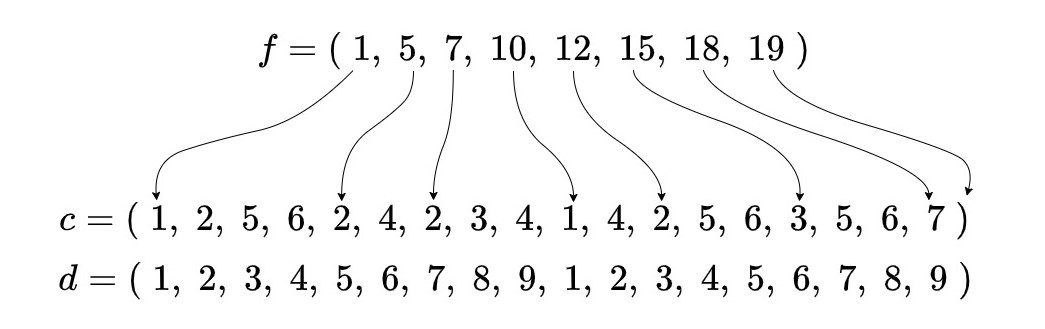
\includegraphics[width=\textwidth]{imagenes/chapter2/csr-format.jpg}
\end{center}
\caption{Matriz $A$ almacenada en formato CRS.}
\label{crs-matrix}
\end{figure}


En la Figura~\ref{crs-matrix} se muestra cómo se representa la matriz $A$ utilizando la estrategia CRS.
Para acceder al valor $A(i,j)$ de la matriz $A$, se obtienen primero los \'indices $p_1=f(i)$ y $p_2=f(i+1)$, posteriormente se busca el \'indice $p$ tal que $p_1 \leq p < p_2$ y $c(p) = j$, y luego se puede obtener el valor buscado accediendo a $d(p)$. 
 
 Si la matriz tiene más coeficientes no nulos que cantidad de filas, la estrategia CRS utiliza menos memoria que el formato simple. Es necesario conocer todas las posiciones de los coeficientes para generar la estructura en forma eficiente o, dicho de otra forma, es muy difícil agregar un nuevo valor a la estructura, a menos que sean posteriores en la matriz al último elemento ya presente. Este formato permite acceder fácilmente a todos los elementos de una fila, pero no a los de una columna.


\subsection{CCS (Compressed Column Storage)}

 El formato comprimido por columna es similar al CRS pero utilizando el vector comprimido para las columnas.
En la Figura~\ref{ccs-matrix} se muestra como se aplica esta estrategia a la matriz $A$.

\begin{figure}[h]
\begin{center}
\begin{eqnarray*}
d = \left(
\begin{array}{cccccccccccccccccc}
1 & 1 & 2 & 5 & 7 & 3 & 8 & 6 & 6 & 9 & 2 & 3 & 4 & 7 & 4 & 5 & 8 & 9\\
\end{array}
\right)\nonumber\\
f = \left(
\begin{array}{cccccccccccccccccc}
1 & 4 & 1 & 2 & 3 & 5 & 3 & 6 & 2 & 3 & 4 & 1 & 5 & 6 & 1 & 5 & 6 & 7\\
\end{array}
\right)\\
c = \left(
\begin{array}{cccccccc}
1 & 3 & 7 & 9 & 12 & 15 & 18 & 19\\
\end{array}
\right)\nonumber
\end{eqnarray*}
\end{center}
\caption{Matriz A almacenada en formato CCS.}
\label{ccs-matrix}
\end{figure}

 Se mantienen las necesidades de memoria del formato CRS y en cuanto a las características de acceso se invierten los conceptos con respecto  a filas y columnas.
 
\subsection{DIA (DIAgonal format)}\label{dia-format}

 \begin{figure}[h]
     \centering
     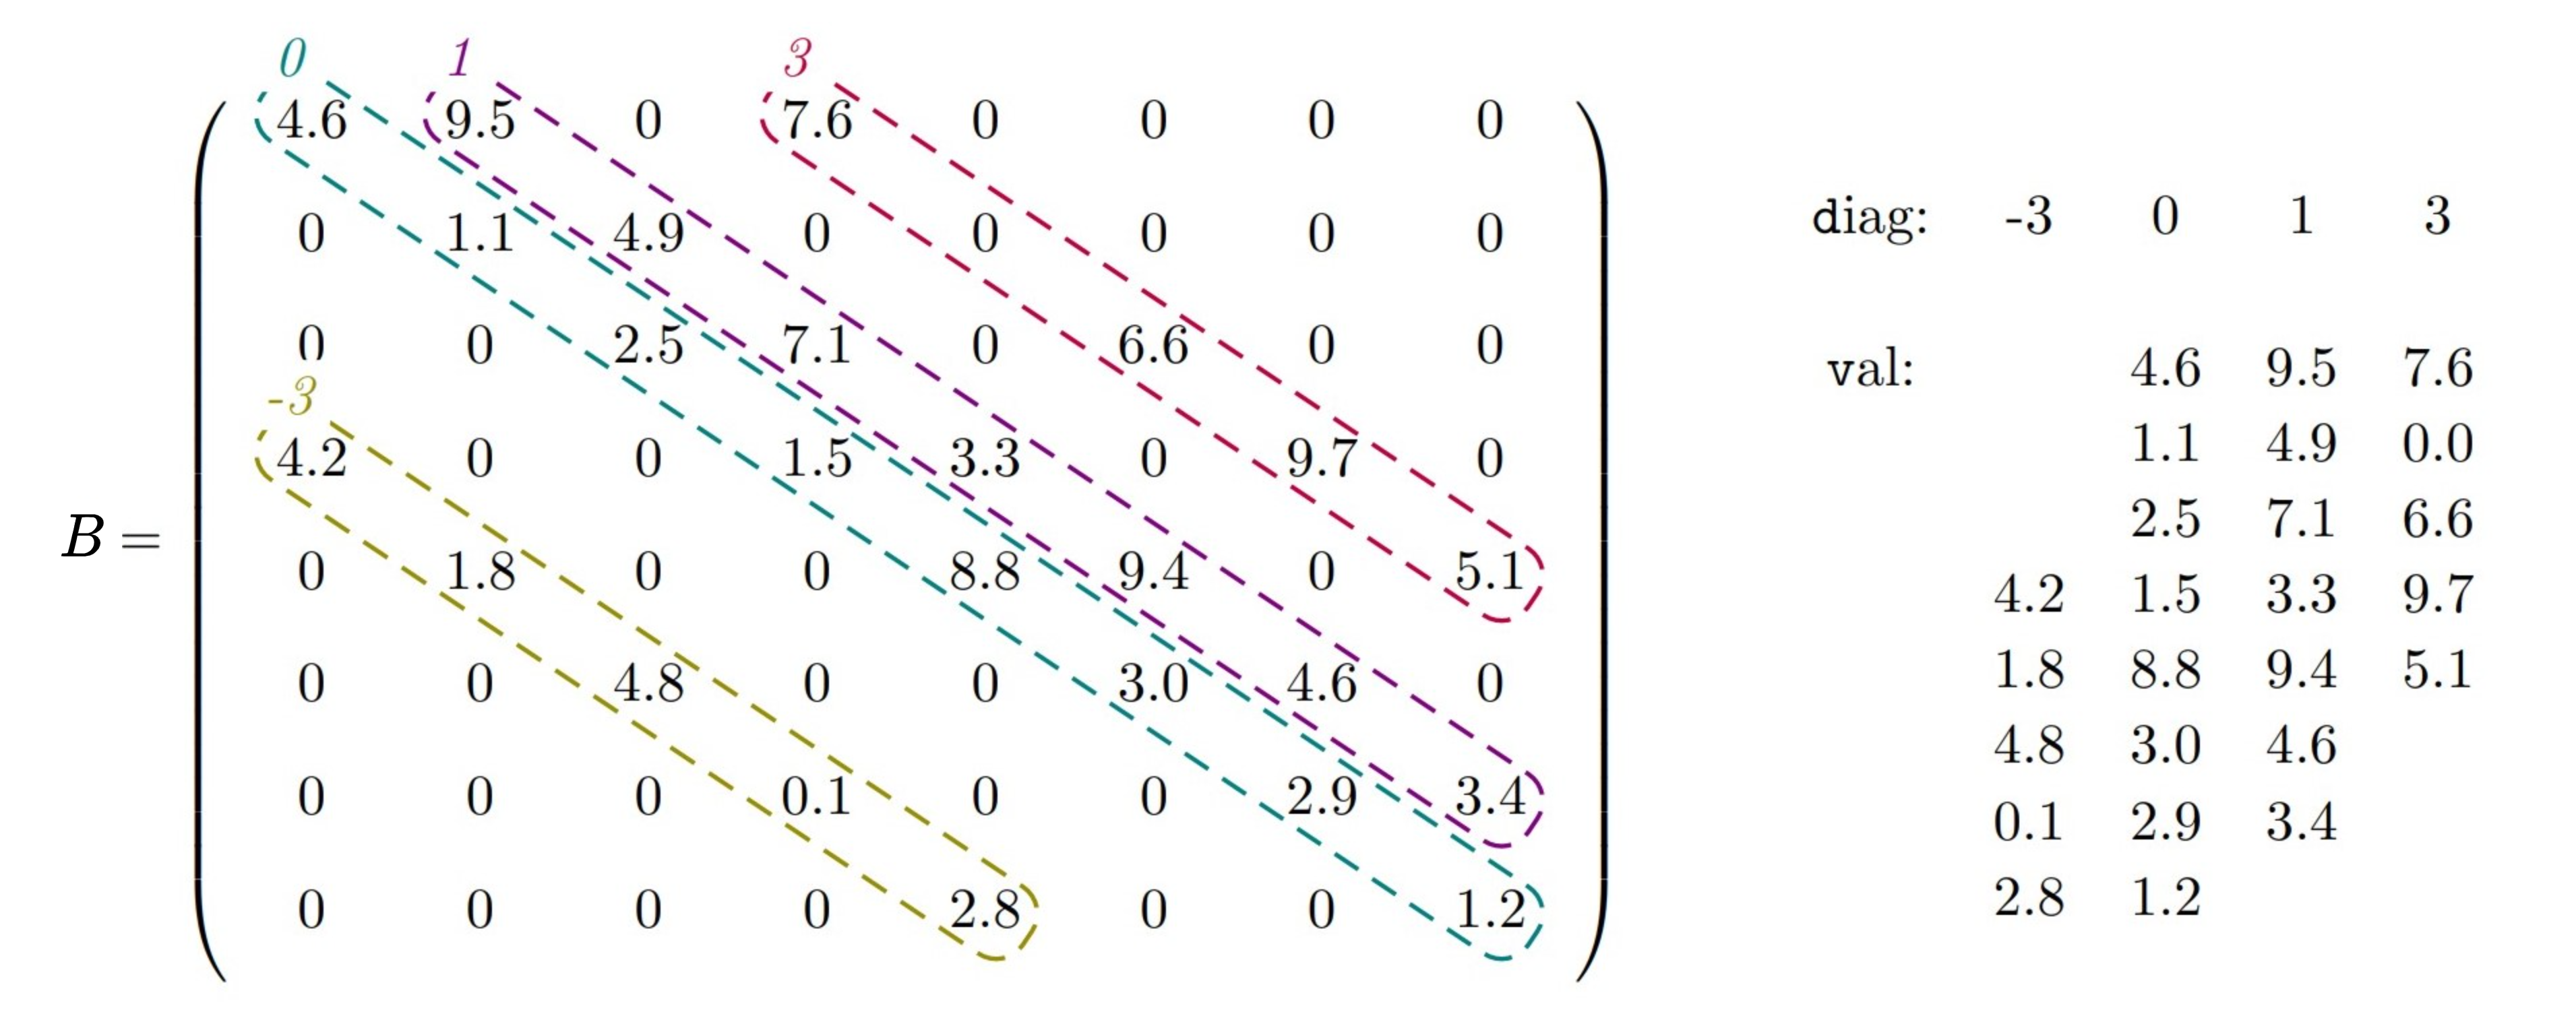
\includegraphics[width=\textwidth]{imagenes/chapter2/diag-format-B.png}
     \caption{Matriz $B$ almacenada en formato DIA.}
     \label{fig:diag-format}
 \end{figure}
 
 
 Cuando la matriz a almacenar es de banda, se pueden utilizar estrategias de almacenamiento por diagonales.
Entonces se almacena la matriz original en una matriz rectangular de tamaño  $n \times d$ siendo $n$ la dimensión de la matriz y $d$ la cantidad de diagonales.


 Si se desea almacenar una matriz que posee $d$ diagonales no consecutivas, % en las que se encuentran los coeficientes distintos de cero pero no siendo las diagonales principales
 una variante de formato es el \textit{DIAgonal storage Format}  que  utiliza una matriz de tamaño $n\times d$ en la que se almacenan las $d$ diagonales y un vector de tamaño $d$ en el que se  especifica el desplazamiento de cada diagonal con la diagonal principal, estando la diagonal principal asociada con 0, las diagonales ``por encima'' con valores positivos y ``por debajo'' con valores negativos. En la Figura~\ref{fig:diag-format} se puede ver un ejemplo.
 


\subsection{ELL (Ellpack-itpack)}\label{ell-format}


En el formato \textit{Ellpack-itpack}, se utiliza una estructura densa de tamaño $n\times k$, donde $n$ es la cantidad de filas y $k = max_i(\nnz(A_i))$, con $A_i$ la fila $i$-ésima de la matriz, es decir, la cantidad máxima de elementos no nulos por fila. La matriz dispersa es almacenada en dos matrices ``densas'' de tamaño $n\times k$, una con las entradas no nulas de la matriz y otra con los índices de las columnas. Es necesario agregar explícitamente valores nulos para completar la primer matriz (\textit{zero padding}). Este problema es menor cuando todas las filas de la matriz son de largos similares (el caso ideal son las matrices con cantidad constante de elementos por fila/columna). En la Figura~\ref{fig:ell-matrix}, se puede observar como se almacena una matriz en formato ELL.

Dado que la estructura elegida es de tamaño $n \times k$, es decir, tiene la misma cantidad de filas que la matriz original, no es necesario almacenar explícitamente los índices de fila ya que están implícitos en la estructura, a diferencia de otros formatos, como por ejemplo COO.

% TRABAJANDO EN IMAGENES MEJORES

% EL PORQUE DEL HYB (hybrid format propuesto por  Bell and Garland)
% Este formato es poco eficiente cuando la cantidad de elementos no nulos en cada fila varia considerablemente respecto al promedio de elementos no nulos por fila. Dado el caso, hay una pérdida en términos del espacio necesario para almacenar la matriz, asi como 
% \begin{figure}
%     \centering
%     \begin{eqnarray*}
%     \left(
%     \begin{array}{ccccccc} 
%     1 & 2 & 3 & 4 \\
%     5 & 6 & 0 & 0 & 0\\
%     7 & 8 & 9 & 0 & 0 & 0\\
%     1 & 2 & 0 & 0 & 0\\
%     3 & 4 & 5 & 0 & 0\\
%     6 & 7 & 8 & 0 & 0 & 0\\
%     9 & 0 & 0 \\
%     \end{array}
%     \right)
%     \end{eqnarray*}
%     \caption{Matriz $A$ en el formato ELL (INCOMPLETO).}
%     \label{fig:ell-matrix}
% \end{figure}

\begin{figure}
    \centering
    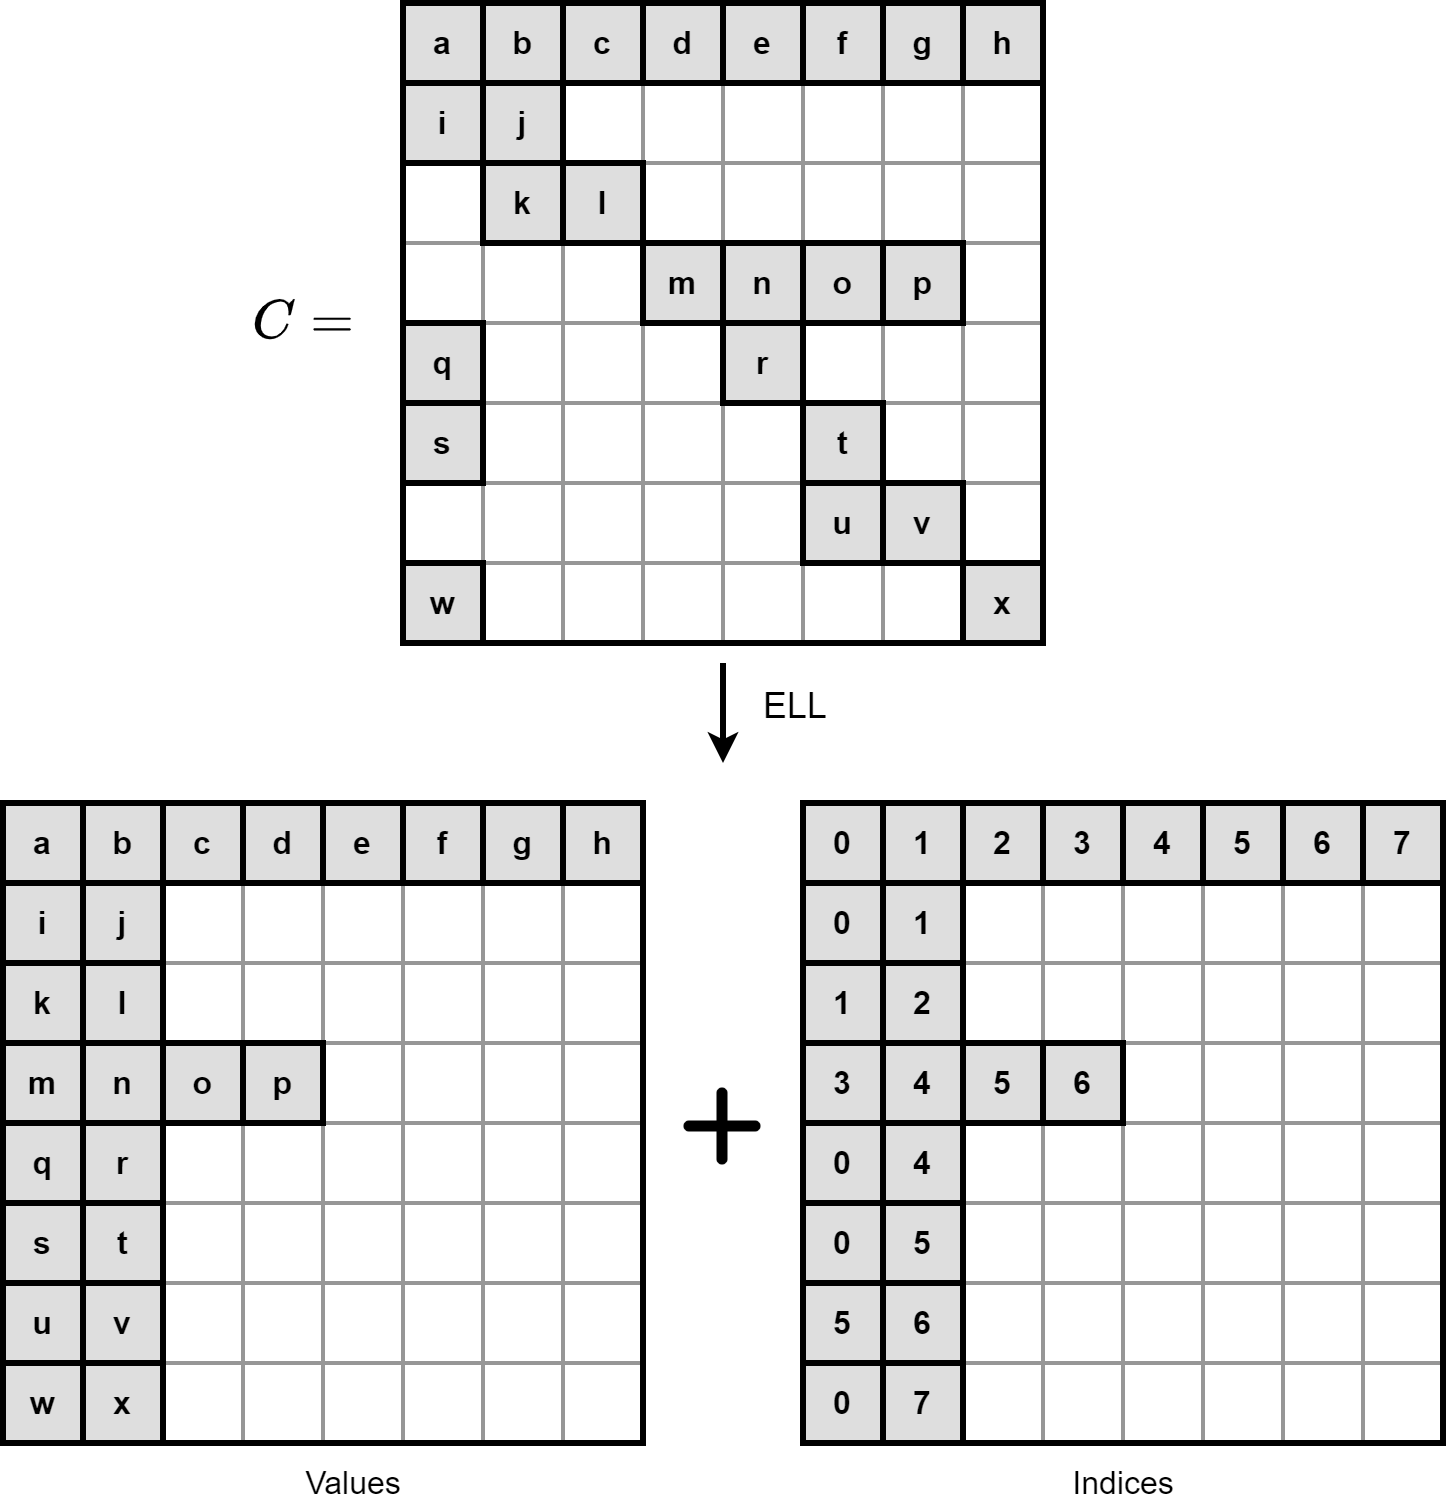
\includegraphics[width=0.7\textwidth]{imagenes/chapter2/ell.png}
    \caption{Matriz $C$ almacenada en formato ELL.}
    \label{fig:ell-matrix}
\end{figure}


\subsection{BCRS (Block Compressed Row Storage)}\label{bcrs}

\begin{figure}
    \centering
    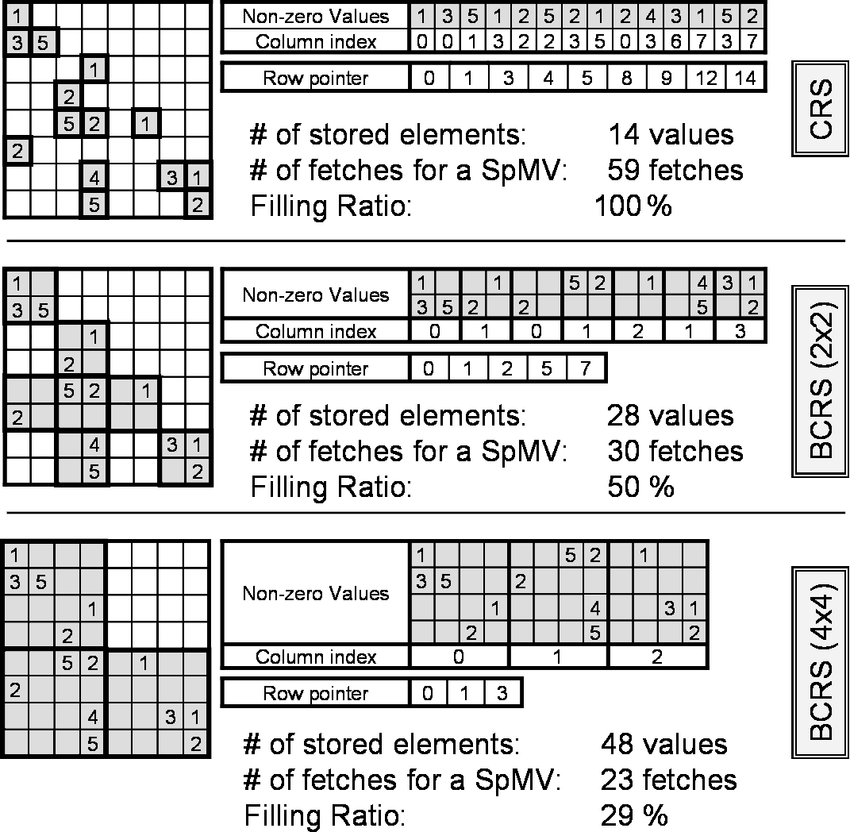
\includegraphics[width=\textwidth]{imagenes/chapter2/bcrs.png}
    \caption{Ejemplo de matriz almacenada en formato BCRS aplicado con distintos tamaños de bloque y comparación con CRS. Extraído de \cite{Buatois2009}.}
    \label{fig:bcrs}
\end{figure}

Este formato se utiliza cuando la matriz se puede dividir/almacenar eficientemente como sub-bloques regulares.

Se tiene entonces, una matriz de $n \times m$ con $nnz_b$ bloques de dimensión $n_b$\footnote{En general los bloques son cuadrados y tanto $m$ como $n$ son múltiplos de $n_b$.}, con entradas de números en punto flotante, enfocada a almacenar los elementos no nulos, además de dos vectores de números enteros, uno para el índice de columna de cada sub-bloque y el otro con el índice (puntero) al comienzo de cada fila.

Notar que este formato funciona razonablemente bien si la matriz posee bloques regulares.

\subsection{BCCS (Block Compressed Column Storage)}\label{bccs}

Funciona de la misma manera que BCRS pero, a la hora de acceder a cada sub-bloque de la matriz, se utiliza CCS.

%\subsubsection{JDS}
%\subsubsection{SKS}



% \subsection{Estrategias Dinámicas}
% %  Las distintas estrategias din\'amicas generalmente utilizan punteros para implementar las estructuras, por lo tanto para implementar las  variantes es necesario utilizar lenguajes que soporten \texttt{allocate} din'amico por ejemplo \texttt{C} y \texttt{Fortran 90}.
% Este tipo de formatos no son de uso común en el álgebra lineal numérica, al menos en las últimas décadas, y su uso es más difundido en campos como las bases de datos. Se incluyen en la revisión por completitud. 
\subsection{LLRCS (Linked List Row-Column Storage)}

En esta estrategia se utiliza una multi-estructura bidimensional. 
Cada entrada correspondiente a un no-nulo contiene dos punteros a sus adyacentes por
fila, y dos a sus adyacentes por columna. Además, dispone de dos vectores de tamaño igual a la cantidad de filas y columnas,  
% en cada entrada se dispone de un puntero para recorrer  las distintas entradas por fila en un vector o por columna en el otro.
con punteros al comienzo de cada fila o columna, respectivamente.

La memoria que se necesita para implementar la estrategia LLRCS, si \nnz es la cantidad de coeficientes no nulos,  se necesitan \nnz posiciones de  punto flotante, $4\ \times\ $\nnz punteros, \nnz enteros, más la memoria necesaria para almacenar los dos vectores ($2 \times n$ punteros).

 Para acceder al valor $A(i,j)$ se puede recorrer la lista de la entrada $i$ por el vector de filas buscando el valor cuya columna sea $j$, o recorrer la lista de la entrada $j$ del vector de columnas hasta encontrar la fila $i$. 
%\pagebreak

\subsection{LLRS (Linked List Row Storage)}

 En esta estrategia se utiliza una estructura unidimensional, en la cual se emplea un vector de tamaño igual a la cantidad de filas, y de cada posición del vector se puede obtener la lista de entradas de esa fila.
 
 En cuanto a memoria, se necesitan \nnz posiciones de punto flotante, \nnz enteros, \nnz  punteros, más el vector de entrada ($n$ punteros). 


\subsection{LLCS (Linked List Column Storage)}

Al igual que en la propuesta anterior, en la estrategia LLCS se utiliza una estructura unidimensional, pero el vector base de la estructura es de tamaño igual a la cantidad de columnas y de cada posición del vector se puede obtener la lista de coeficientes no nulos de esa columna. La estrategia LLCS posee las mismas necesidades de memoria que la LLRS.



\section{Multiplicación Matriz-Vector (SpMV)}\label{spmv}

Si bien el objetivo del proyecto no se centra en estudiar las matrices dispersas para una operación particular, la importancia que implica la operatoria al trabajar con éstas obliga a mostrar algunas operaciones específicas. Por esta razón, en este apartado se presenta la multiplicación Matriz Dispersa-Vector (SpMV por su nombre en Inglés Sparse Matrix-Vector). La SpMV \cite{golub1996matrix} es una operación de la forma $y = Ax$, donde $A$ es una matriz dispersa de tamaño $m\times n$, los vectores $x$ e $y$ son densos de tamaño $n$ y $m$ respectivamente. Este kernel es altamente utilizado y con enormes aplicaciones en la computación científica. Dada su importancia, la implementación de esta operación ha sido fuertemente estudiada  en variedad de contextos, desde diferentes formatos dispersos, hasta diversas arquitecturas de hardware, entre ellas: GPUs, FPGAs e incluso en dispositivos como TPUs~\cite{Ku2008,Reguly2012,He2020}. %Si bien la carga computacional de esta operación no es elevada, debido a que la matriz es dispersa y la multiplicación por los coeficientes nulos no es necesaria computarla, 

Si bien las operaciones necesarias para su cómputo son simples (sumas y multiplicaciones), la SpMV, presenta ciertas limitantes a la hora de su ejecución.
El cuello de botella se da en los accesos a memoria (principalmente por la aleatoriedad de los accesos). 
Este hecho ha motivado que muchos esfuerzos por optimizar la SpMV se centren en definir formatos de almacenamiento adecuados. Esto ha permitido que en muchas de las implementaciones de la operación SpMV, los accesos a la matriz $A$ sean ordenados y bien aprovechados, obteniendo accesos predecibles y eficientes. Mientras que, en general, el vector $x$ es accedido de forma irregular debido a la estructura de la matriz $A$, sacando poco beneficio de la localidad de datos y desaprovechando del uso de memorias cache. %(Posibles planteos para mejorar dichos accesos :reducir el ancho de banda de la matriz, dando accesos mucho mas coalesced, estrategia a evaluar en el correr del proy. aplicando por ejemplo RCM)

A modo de ejemplo, en el Algoritmo~\ref{alg:CSR_serial}, se presenta en alto nivel el procedimiento secuencial que computa SpMV, utilizando el formato CSR para almacenar la matriz $A$. El primer ciclo \texttt{for} ($i$) recorre las filas de la matriz $A$, y el segundo \texttt{for} interno ($j$) calcula, accediendo a los elementos no nulos almacenados en $d$ a través de los punteros en $f$, para cada fila, la multiplicación por los coeficientes correspondientes del vector~$x$ (accedido en las posiciones donde existen elementos no nulos indicado por $c$) y se almacena el resultado en la posición del vector~$y$ pertinente.

\begin{algorithm}[th]
\textbf{Input:} $f, c, d, x$ \\
\textbf{Output:} $y$
\begin{algorithmic}
\STATE{$y = 0$}
%\STATE{in parallel...}
\FOR{$i = 1$ \TO $m$}
\FOR{$j = f[i]$ \TO $f[i+1]-1$ }
\STATE{$y[i] = y[i] + d[j] \cdot x[c[j]]$}
\ENDFOR
\ENDFOR
\end{algorithmic}
\caption{
% Serial computation of sparse matrix-vector multiplication (SpMV) with the sparse matrix $A$ stored in the CSR format.
% The vector $d$ stores the nonzero values of $A$ by rows;  $f$ contains the indexes that specify the first element %correspond to the beginning
% of each row in vector $d$; and $c$ contains the column index of each element in the original matrix.
% The nonzero elements within each row are ordered by column index.
% %Typical procedure of the \spmv for the CSR sparse storage format.
Cálculo secuencial de la multiplicación matriz dispersa-vector (SpMV) con la matriz dispersa $A$ almacenada en el formato CSR. 
El vector $d$ almacena los valores distintos de cero de A por filas, $f$ contiene los índices que especifican el primer elemento de cada fila en el vector $d$; y $c$ contiene el índice de columna de cada elemento en la matriz original. 
Los elementos distintos de cero dentro de cada fila están ordenados por índice de columna.
}
\label{alg:CSR_serial}
\end{algorithm}


\section{Estrategias de reordenamiento}\label{sec:reordenamientos}

% \resumen{Por que reordenar}

Como se menciona en las secciones anteriores, muchas de las matrices dispersas con las que se trabaja en la actualidad corresponden a discretizaciones de problemas de redes eléctricas y distribución de energía, ingeniería estructural, etc. y, más en general, formulaciones de sistemas de ecuaciones diferenciales parciales. Estos sistemas son aproximados mediante ecuaciones con una cantidad finita de incógnitas, y resultan en sistemas de la forma $Ax = b$, con $A$ una matriz dispersa.
Buscando explotar estas características, por muchos años, la estrategia más difundida fue intentar llevar las matrices a una matriz equivalente pero de banda. Notar que, una matriz con un ancho de banda pequeño es útil principalmente por dos razones. La primera es que permite utilizar una estructura de datos simple en métodos directos como la factorización LU para resolver sistemas lineales dispersos. Segundo, también es útil en métodos iterativos como el método del Gradiente Conjugado, porque los elementos distintos de cero serán agrupados cerca de la diagonal, mejorando así la localidad de los datos. 

%\resumen{Que es reordenar}

En este contexto se desarrollaron las técnicas de reordemaniento para las matrices dispersas. Reordenar es encontrar una permutación $p$ que se aplica tanto para filas como para las columnas de la matriz. Este reordenamiento puede buscar diferentes objetivos. Dada una matriz simétrica $A$, un reordenamiento de reducción de ancho de banda apunta a encontrar una permutación $P$ de modo que el ancho de banda de $PAP^t$ sea pequeño (en el ideal, mínimo). 

Notar que en los problemas que provienen de estructuras de grilla, reordenar la matriz es equivalente a renumerar los nodos de la grilla. Este aspecto también ha sido especialmente abordado en dicho campo de estudio (la generación de grillas de discretización).


%\resumen{el por que de las heurísticas, definir heurística???}

Dado que el problema de encontrar el reordenamiento que minimice el ancho de banda para una matriz es un problema $\mathcal{NP}$-completo~\cite{Papadimitriou1976}, se ha trabajado en estudiar e implementar múltiples heurísticas con el objetivo de encontrar buenas soluciones con esfuerzos computacionales razonables. Una familia importante de estos algoritmos, trata la reducción del ancho de banda de una matriz, como se dijo antes, bajo la perspectiva de un problema de etiquetado de grafos. De esta manera, el problema de reordenar una matriz dispersa $A$ equivale al de etiquetar los vértices o nodos del grafo correspondiente a interpretar $A$ como la matriz de adyacencia asociada. Esto es interpretar cada fila o columna $i$ como un nodo de un grafo, y cada entrada no nula $j$ de dicha fila como una arista que conecta el nodo $i$ con el $j$, tal como muestra la Figura~\ref{fig:adjacency-matrix}. %(SEGURO SE PUEDE REDACTAR MRJOT O ESCRIBIR EN LENGUAJE MAS MATEMATICO con G(V,E) V = 1..n y E = (i,j) tal que $a_ij$ disitnto de 0, que me recomendas?)

\begin{figure}
    \centering
    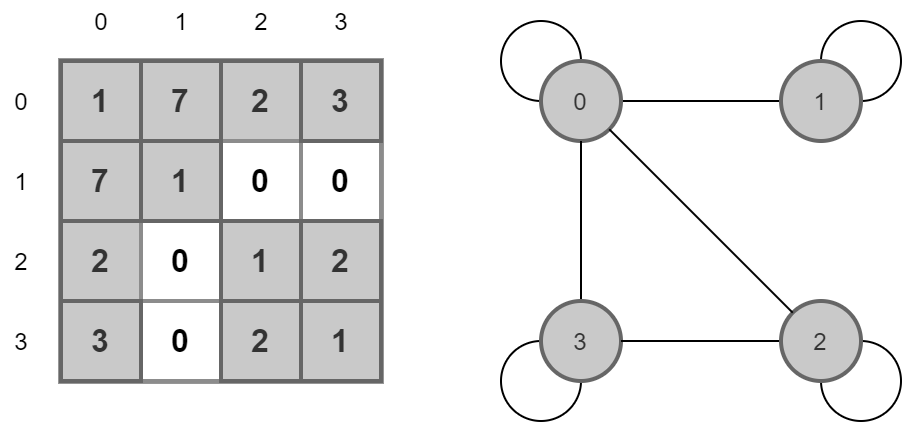
\includegraphics[width=0.6\textwidth]{imagenes/chapter2/adjacency-matrix.png}
    \caption{Ejemplo de grafo y su matriz de adyacencia correspondiente.}
    \label{fig:adjacency-matrix}
\end{figure}  

% 1. Una de las razones por las cuales se aplican estrategias de reordenamiento sobre las filas y columnas de una matriz, es para reducir la cantidad de \textit{fill-in} (DEFINIR EN ALGUN LADO) que crea la factorización, reduciendo así el tiempo y el costo de almacenamiento de los cálculos posteriores.
% 2. Otra de las razones para reordenar matrices dispersas es para reducir los accesos a memoria en durante SpMV. Aplicando re-ordenamientos que reduzcan el ancho de banda (RCM GPS), permite en algunos casos poder almacenar dicha matriz en un formato que aproveche estas características (DIA).


A continuación, son presentadas las heurísticas clásicas para la reducción del ancho de banda, Cuthill-McKee (CM)~\cite{Cuthill-Mckee}, Reverse Cuthill-McKee (RCM)~\cite{alan-phdthesis} y Gibbs-Poole-Stockmeyer (GPS)~\cite{Gibbs1976}. Es preciso mencionar que, a pesar que estas herramientas funcionan relativamente bien, no hay que dejar de lado que son  heurísticas, por lo tanto no son métodos que garanticen alcanzar la solución óptima, sino que una solución aceptable buscando un buen balance costo/beneficio.

 \subsection{Cuthill-McKee (CM)}\label{CM}

El algoritmo de Cuthill-McKee~\cite{Cuthill-Mckee}, está basado en la aplicación de una estrategia de recorrida Breadth-First-Search (BFS), en la que el grafo asociado a la matriz es atravesado por niveles, determinados a partir del nodo raíz (nivel 0). A medida que se atraviesan los nodos de un nivel, a estos se los marca y numera en base al orden en que son recorridos. A continuación, se inspeccionan los vecinos de cada uno de estos nodos marcados, cada vez que se encuentra un vecino de un nodo visitado que no está numerado, se lo agrega a una lista y se etiqueta como el siguiente elemento del siguiente nivel. El orden en el que se atraviesa cada nivel da lugar a diferentes ordenamientos o permutaciones de filas y columnas. En el proceso de reordenar, en el algoritmo Cuthill-McKee, los nodos adyacentes a un nodo visitado siempre se atraviesan del grado más bajo al más alto.


\begin{algorithm}[]
%\SetAlgoLined
\textbf{Input:} Grafo $G$ \\
\textbf{Output:} $p$



 $v_1 \leftarrow r$; // Nodo inicial o raíz, en algunos casos el de menor grado - nodo periférico  \
 
 \For{$i = 1$ \KwTo $n$}{
  Encontrar todos los nodos adyacentes de $v_i$ sin numerar\; %Find all the unnumbered neighbors of the vertex $v_i$\;
  Etiquetar los nodos encontrados en orden creciente de grado\; %Label the vertices found in increasing order of degree\;
%   \eIf{condition}{
   
%   }{
%   instructions3\;
%   }
 }
 \caption{Cuthill-McKee. Esquema general en alto nivel del algoritmo Cuthill-McKee.}
 \label{alg:cm}
\end{algorithm}

\subsection{Reverse Cuthill-McKee (RCM)}\label{RCM}
Variante del algoritmo CM, anteriormente descrito, en el que se ``invierte'' el orden obtenido para las filas/columnas.
La heurística RCM produce como resultado matrices con el mismo ancho de banda que CM, pero con \textit{profile} menor.

En la versión original de la heurística RCM propuesta por Alan George, también son seleccionados como vértices iniciales aquellos con grado mínimo en el grafo y se generan las estructuras de nivel desde estos vértices.

Las reducciones de ancho de banda y profile de la matriz resultante, obtenidas por las heurísticas CM y RCM, dependen fuertemente de la elección del vértice inicial. Por esto se han realizado varios estudios de como elegir el vértice inicial de manera de lograr optimizaciones en el proceso de encontrar ordenamientos aceptables.


\subsection{Gibbs-Poole-Stockmeyer (GPS)}

Antes de profundizar en esta heurística, es importante presentar algunas definiciones básicas útiles para la técnica, en especial considerando que los autores utilizan el concepto del grafo asociado a la matriz dispersa.

Definición (\textit{distancia}). La distancia, función definida para dos vértices del grafo $\mathit{d} : V \times V \longrightarrow \mathbb{N}$. Sean $u$ y $v$ vértices, la distancia $\mathit{d}(u,v)$ está dada por el largo del camino mínimo entre éstos.

Definición (\textit{excentricidad}). La excentricidad, definida sobre un vértice del grafo, $\mathit{l} : V \longrightarrow \mathbb{N}$, está dada por $\mathit{l}(v) = max_{v,u \in V}(d(v,u))$.

Definición (\textit{diámetro del grafo}). El diámetro $\Phi(G) = max_{v \in V} (\mathit{l}(v)) = max_{v,u \in V} (d(u,v)) $ del grafo $G(V,E)$ es la mayor excentricidad presente en G.


Gibs, Poole y Stockmeyer posteriormente del surgimiento de las heurísticas CM y RCM, verificaron que éstas heurísticas no eran adecuadas en los casos que la elección del vértice inicial implica un costo computacional grande. En dichas técnicas los vértices iniciales son los de menor grado en el grafo, y luego se generan las estructuras de nivel a partir de éstos. Notar, por ejemplo, que CM y RCM harían un cómputo innecesario en situaciones donde los vértices tienen todos el mismo grado. 

Para comprender el algoritmo GPS, es necesario dar   una definición de nodo o vértice pseudo-periférico:

Definición (\textit{vértice periférico}). Un vértice $v$ es considerado periférico si su excentricidad es igual al diámetro del grafo, i.e.  $\mathbf{l}(v) = \Phi(G)$.
Entonces, para Gibbs, Poole y Stockmeyer, un vértice es pseudo-periférico si su excentricidad es cercana al diámetro del grafo. 

En GPS, en lugar de construir varias estructuras de nivel, como en las planteadas en CM y RCM,  sólo se construyen dos (con nodos raíces dos vértices pseudoperiféricos). Gibbs, Poole y Stockmeyer, fueron los primeros autores en utilizar un vértice pseudo-periférico como inicial para la renumeración. Las bondades que ofrece elegir un vértice pseudo-periférico como vértice inicial para renumerar se dan debido a que en la estructura de nivel formada desde este vértice habrá mayor cantidad de niveles y, en consecuencia, menos ancho por nivel, comparado con un vértice que no está en la periferia o cerca de la periferia del grafo de adyacencia.

La heurística GPS se puede dividir principalmente en tres etapas. 
En el primer paso de la heurística GPS, se seleccionan dos nodos pseudo-periféricos, $v, u \in V$, y sus estructuras de nivel asociadas $\mathit{L}(v)$ y $\mathit{L}(u)$, respectivamente, tomando a estos como raíz.
En la segunda etapa de la heurística GPS, en base a las estructuras anteriormente mencionadas en la etapa uno, $L(v)$ y $L(u)$, se crea una nueva estructura de nivel, $K(v, ...)$. Se combina las estructuras de nivel con el objetivo de reducir el ancho por nivel (que sería equivalente al ancho de banda). Este paso asegura que el ancho de nivel de la estructura $K (v, ...)$ sea, como máximo, el ancho de nivel más pequeño de las estructuras de nivel $\mathit{L}(v)$ y $\mathit{L}(u)$.
Finalmente, en el último paso, se renumeran los vértices atravesando la estructura del nivel $K(v, ···)$ generada en la segunda etapa de la heurística GPS. Los niveles se recorren en orden inverso, es decir, desde el nivel $K_{l(v)}(v, ...)$ hasta el nivel $K_{0}(v, ...)$. Esta renumeración se realiza nivel a nivel de la estructura generada, en la que la renumeración de los vértices se realiza en orden ascendente de grado. 



\subsection{Algoritmo Sloan (Sloan)}

%\resumen{El Algoritmo Sloan utiliza pesos, con los que calcula una cierta prioridad entre los nodos, me pareció interesante la técnica}

El algoritmo Sloan~\cite{Sloan1986} es una heurística planteada por Scott W. Sloan en el año 1986 para reordenar matrices dispersas. Normalmente, se utiliza para acelerar el cálculo de sistemas de ecuaciones lineales dispersos como muchas de las otras heurísticas de reordenamientos. 

La idea principal del algoritmo es numerar los vértices desde un punto cercano al diámetro del grafo, un pseudo-diámetro%, manteniendo (en la medida de lo posible) este valor a través del ordenamiento
. En el primer paso, se busca un pseudo-diámetro del grafo y se eligen $s$ y $e$ como extremos de dicho camino. En el paso dos, a cada vértice del grafo se le asocia una cierta prioridad, en base al pseudo-diámetro anterior y al grado de éste, inmediatamente, el vértice inicial $s$ se ordena primero. Luego, en cada etapa, se elige el siguiente vértice a numerar entre el conjunto factible con la mayor prioridad. Manteniendo así, un equilibrio entre los objetivos de mantener un \textit{profile} pequeño y la incorporación de vértices elegibles que se han quedado atrás (lejos de $e$). La lista de vértices posibles para numerar en cada iteración, está formada por los vecinos de uno o más vértices ya renumerados y los vecinos de estos.
 
 El algoritmo, puede entonces, dividirse principalmente en dos fases bien distintivas: (1) selección del vértice inicial $s$ y final $e$, y (2) reordenamiento de vértices.% A esta altura, es clara la importancia de la elección de los vértices iniciales, etapa a la que se le da prioridad en los diferentes algoritmos de reordenamiento. Continuando con el algoritmo,  

Para la prioridad de cada nodo, se utilizan dos pesos positivos $W_1$ y $W_2$ de forma de ponderar las dos propiedades que determinan la prioridad del nodo, en este caso son la distancia al nodo inicial y el grado, respectivamente. 
$P(n) = W_1\times distance(n,s) - W_2\times degree(n)$.

\begin{algorithm}[]
\textbf{Input:} Grafo $G$, Pesos $W_1, W_2$, Nodos $s,e$ \\
\textbf{Output:} $p$
\begin{algorithmic}
% \COMMENT{Inicializar los vertices}
\STATE nextId = 0;
\FOR{\textbf{each} $n$ Node \textbf{in} G}
\STATE{status(n) = inactive;}
\STATE priority(n) = $W_1 \times$ distance(n,s) - $W_2 \times$ degree(n);
\ENDFOR

\STATE status(s) = preactive;
\STATE working\_queue = \{s\};

\FOR{\textbf{each} $n$ node \textbf{in} working\_queue \textbf{order by} priority}
\FOR{\textbf{each} $v$ \textbf{in} Neighbors($n$)}
\IF{status(n) == preactive \AND (status(v) == inactive \OR status(v) == preactive))}
    \STATE update(priority(v));
    \STATE status(v) = preactive;
    \STATE updateFarNeighbors(v,working\_queue);
\ELSIF{status(n) == preactive \AND status(v) == active)}
    \STATE update(priority(v));
\ELSIF{ status(n) == active  status(v) == preactive)}
    \STATE update(priority(v));
    \STATE status(v) = active;
    \STATE updateFarNeighbors(v,working\_queue);
\ENDIF
\STATE p[nextId++] = n;
\STATE status(n) = numbered;
\ENDFOR
\ENDFOR

\FOR{$i = 1$ \TO $m$}
\FOR{$j = f[i]$ \TO $f[i+1]-1$ }
\STATE{$y[i] = y[i] + d[j] \cdot x[c[j]]$}
\ENDFOR
\ENDFOR
\end{algorithmic}
\caption{
Algoritmo Sloan. Pseudocódigo para una posible implementación secuencial del algoritmo Sloan. Extraído de~\cite{sloan-parallel}.
}
\label{alg:sloan-serial}
\end{algorithm}

El Algoritmo~\ref{alg:sloan-serial} presenta un pseudocódigo de cómo funciona el algoritmo Sloan. En cada iteración, los  nodos del grafo puede estar en uno de 4 estados: (i) \textit{numerado}, (ii) \textit{activo}, (iii) \textit{preactivo}, para los nodos vecinos de algún nodo activo, y un cuarto estado (iv) \textit{inactivo} para el resto de los nodos. Inicialmente, sólo el nodo inicial $s$ está en estado \textit{preactivo} mientras que el resto se encuentra en estado \textit{inactivo}. Seguido, el algoritmo itera a través de todos los nodos del grafo, y en cada paso elige entre los nodos \textit{activos} o \textit{preactivos} en orden descendente de prioridad, es decir, maximizando en cada paso la prioridad. Posteriormente, se asignan nuevas prioridades a los vecinos y los vecinos de éstos son seleccionados para procesar.

Existen también, implementaciones en paralelo para este algoritmo, tal y como se  plantea en~\cite{sloan-parallel}.

%(Pueden haber otros ordenamientos, que no busquen reducir el ancho de banda, sino el fill in producido a la hora de operar, por ejemplo en métodos iterativos x exactos ???). Parrafo diciendo que tambien se usa para otras cosas.....


\newpage\section{Plataformas de hardware heterogéneas en HPC}

% \resumen{intro feneral para arquitect de hpc}

La computación de alta performance (HPC), al día de hoy, es una de las herramientas más importantes para el avance de la computación científica. 
El desarrollo tecnológico ha motivado resolver problemas más grandes y/o con mayor precisión. Esto, a su vez, se retro-alimenta y genera aún mayores necesidades computacionales. En este contexto, la HPC aporta en soluciones tecnológicas que sirven de base para abordar este tipo de realidades. Entre otros campos, el uso de HPC ha permitido el desarrollo de áreas %Como se ha mencionado anteriormente, así como las matrices dispersas modelan tantos problemas científicos complejos, con las arquitecturas y el hardware enfocado al HPC, se buscan resolver, 
como el pronóstico del tiempo, la exploración de energía, la bioinformática~\cite{hpc-bioinformatics}, el % hasta la dinámica de fluidos computacional, combinar simulaciones tradicionales con inteligencia artificial, 
aprendizaje automático, el análisis de big data~\cite{big-data2015} y el edge-computing~\cite{Tu2019}.


Entre las arquitecturas de hardware utilizadas para la HPC se encuentran las unidades de procesamiento gráfico, o GPU (del inglés Graphics Processing Units). Son coprocesadores diseñados originalmente para alivianar la carga de la CPU en aplicaciones con una importante carga de trabajo dedicada a la representación de gráficos en la pantalla, como pueden ser videojuegos o simulaciones con un alto contenido de imágenes 3D, entre otras cosas~\cite{Kirk2013}. 
En los últimos años, los avances tanto en el hardware como en distintos lenguajes de programación orientados a estas arquitecturas, que permiten, no sólo trabajar con procesamiento gráfico, sino que también con problemas de propósito general como simulaciones y modelos numéricos. Entre los lenguajes orientados a este tipo de arquitecturas se destaca \texttt{CUDA} (estándar de bibliotecas de la empresa \texttt{Nvidia}). Gracias a la programabilidad y flexibilidad de la arquitectura \texttt{CUDA}, las GPU han pasado a ser verdaderos procesadores masivamente paralelos, presentes en la mayoría de las plataformas de HPC modernas.
Debido a la gran importancia que han tenido las GPUs en la computación científica, y en particular en el ALN, se dedica la Sección~\ref{sec:gpu-arch} al estudio de su arquitectura.
% Este desarrollo transforma a las GPUs en verdaderos procesadores masivamente paralelos, ofreciendo altos niveles de cómputo.



\subsection{Arquitectura de las GPUs}\label{sec:gpu-arch}
% Es normal comparar el rendimiento de las GPUs frente a las CPUs, las grandes ventajas que estas poseen frente a los procesadores mas utilizados.

% A continuación se intenta explicar el porque de la gran importancia de las GPUs frente a los problemas de computación y la 
% A continuación se explica la arquitectura y una comparación entre GPUs y CPUs



% ACA HABLAR DE LA LIMITANTE O BARRERA FISICA CON LA QUE SE ENCUENTRAN UTILIZANDO EL ENFOQUE DE AUMENTAR LA CANTIDAD DE CICLOS U OPERACIONES QUE EL PROCESADOR PODRIA HACER SECUENCIAMENTE POR SEGUNDO I.E. LA FRECUENCIA DEL RELOJ. ESTO DIRIGIA A UN AUMENTO DE LA TEMPERATURA (NO ENCONTRE SI ES LINEAL O EXPONENCIAL, PROBABLEMENTE EXPONENCIAL), LO QUE DISPARABA LOS COSTOS ENERGETICOS. CAMBIANDO EL PARADIGMA, SE APLICA LA IDEA DE TENER MAS PROCESADORES TRABAJANDO AL MISMO TIEMPO, PERO A FRECUENCIAS MAS BAJAS

% \resumen{TENGO PENDIENTE MODIFICAR UN POCO BASTANTE ESTA SECCION PARA QUE NO SEA TAN GPU porque no esta enfocada tanto en gpu.... Y MAS HPC}


En el año 1965 Gordon Moore planteaba la tan conocida Ley de Moore, en la que afirmaba, a grandes rasgos, que la cantidad de transistores dentro de los microprocesadores se duplicaría en el período de 2 años, fenómeno que se ha ido cumpliendo hasta el día de hoy.
Si se observa la evolución de los procesadores CPU, durante el período comprendido entre los años 70-80 hasta el 2004, el número de cores dentro del procesador no presentó cambios, en particular se mantuvo en uno. Esto se debe, principalmente, a que la arquitectura de la CPU estaba pensada para ser puramente secuencial, dando lugar a la pregunta de cómo se fue mejorando el rendimiento de los procesadores. Básicamente, la estrategia para mejorar el desempeño de los procesadores, fue aumentar la frecuencia a la que trabajaban, así como la cantidad de transistores en el chip. 
Observando la Figura \ref{fig:42-trend-data}, es posible notar que además de aumentar los transistores y la frecuencia a la que trabajan los procesadores aumenta, de forma conjunta, la potencia utilizada o requerida por los mismos. Esto se debe a que, físicamente, la potencia está directamente  relacionada a la frecuencia así como el voltaje al que trabajan los procesadores, relaciones dadas por la siguientes ecuaciones de proporcionalidad:
\begin{equation*}
P \propto CV^2f,
\end{equation*}
donde $C$ es la carga capacitiva, $V$ el voltaje y $f$ la frecuencia. Básicamente, a mayor frecuencia, dado que son voltajes bajos, la potencia queda en su mayoría determinada por la corriente que circula por el procesador, y a mayor cantidad de carga pasando por un conductor mayor es el calor.

Si bien no se muestra en la Figura \ref{fig:42-trend-data}, a medida que el consumo de potencia iba en aumento junto con la frecuencia, la primer estrategia para reducir el consumo energético de los procesadores fue reducir el voltaje. Se fue disminuyendo, pasando de manejar valores de voltaje en el rango de 5V a 1V. Esto permitió alcanzar frecuencias de alrededor de 3,6 GHz (sin disparar demasiado la potencia o con valores controlables) aumentando razonablemente el rendimiento de los procesadores. Llegado el punto, la reducción de voltaje ya no era viable (debido  a que los 1s y 0s están representados por diferentes voltajes, seguir reduciendo provocaría que estos no puedan ser correctamente distinguidos) y seguir aumentando la frecuencia traía consigo el problema antes mencionado, consumo de potencia y calor disipado, encontrándose con el fenómeno denominado ``The Power Wall''.
\begin{figure}
    \centering
    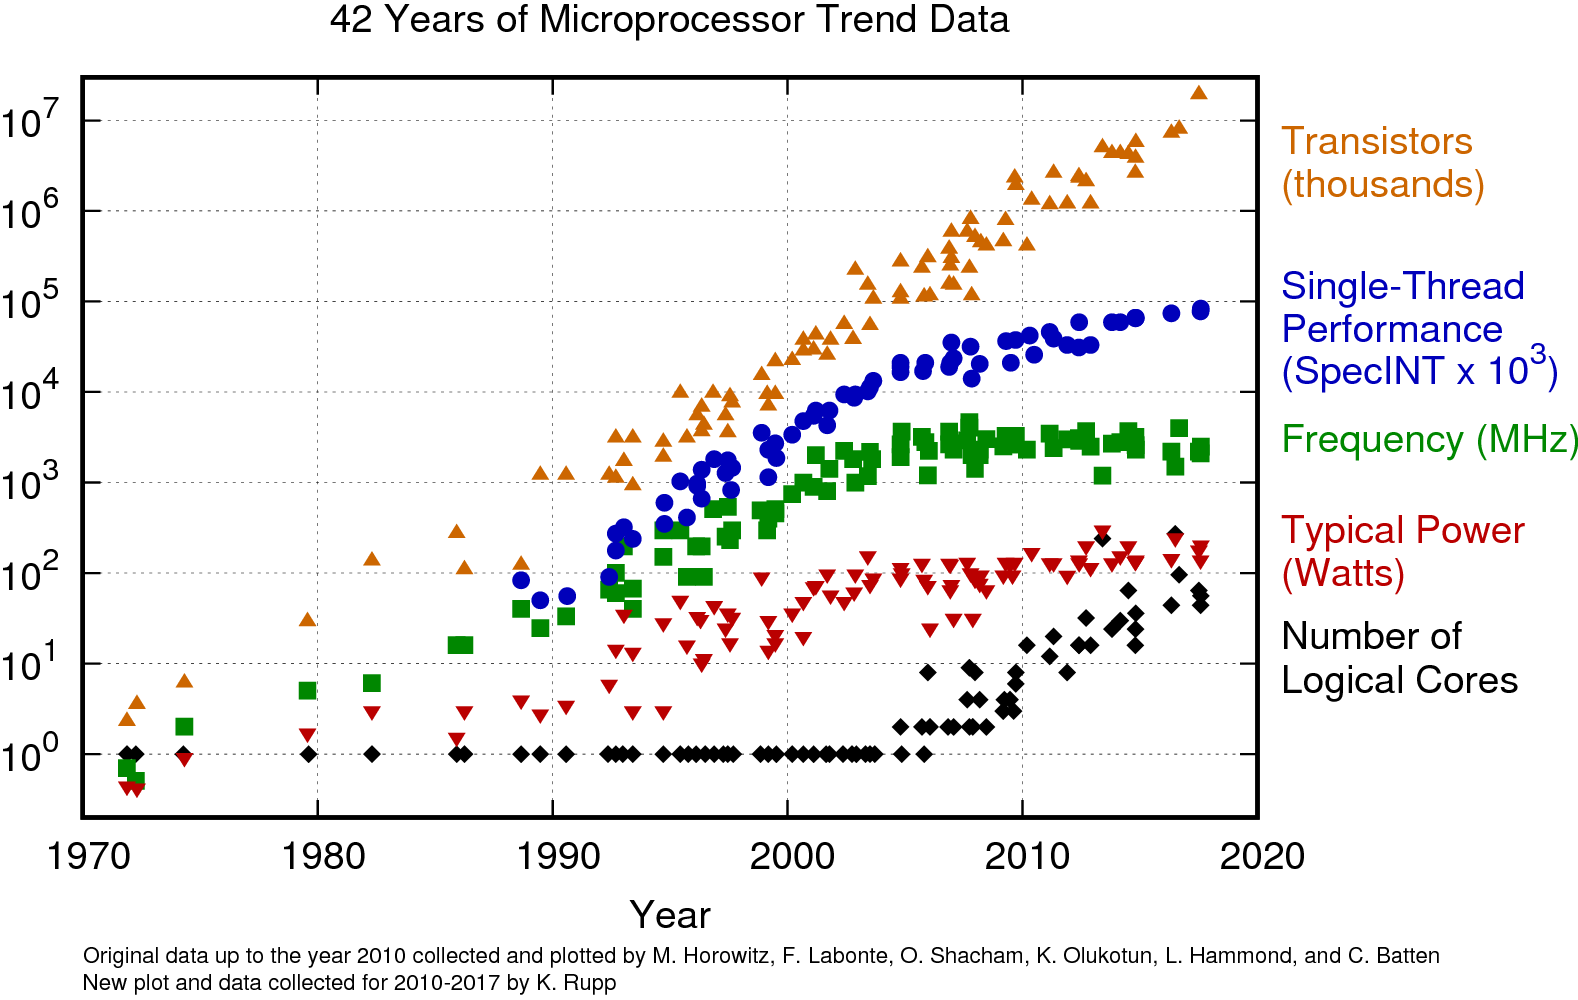
\includegraphics[width=\textwidth]{imagenes/chapter2/42-years-processor-trend.png}
    \caption{Evolución de los procesadores y sus principales factores. Extraído de~\cite{42-trend-data}.}
    \label{fig:42-trend-data}
\end{figure}

Debido a la barrera física con la que se enfrentan en caso de seguir con la misma estrategia, era necesaria la creación de sistemas más sofisticados de enfriamiento, como los que propuso \texttt{IBM} en su momento basados en enfriamiento liquido \cite{ibm-cooling}, lo que motivó la elección de una nueva dirección de desarrollo. Para mitigar y resolver este problema, en lugar de aumentar la frecuencia, se adoptó la idea de aumentar la cantidad de cores dentro del procesador, pero funcionando a frecuencias más bajas. Estrategia mejor conocida como \textit{multicore}, que al día de hoy se mantiene con fuerza siendo así inspiración para las arquitecturas paralelas como la GPU, que explota esta idea en gran escala. En particular, las GPUs han ido agregando más cores (funcionando a frecuencias bajas), entre otros factores que han permitido el aumento de performance de estos dispositivos. Dicha evolución vuelve a estos dispositivos una arquitectura muy atractiva en ámbitos de la computación científica.

La GPU y la CPU presentan grandes diferencias a nivel de arquitectura, ya que en la primera, la gran mayoría de los transistores están dedicados al cómputo mientras que en la última están dedicados a intentar mejorar el tiempo de ejecución secuencial. En una CPU tradicional, gran parte de los transistores están destinados a realizar otro tipo de tareas que el cómputo, como por ejemplo: 

\begin{itemize}
    \item predicción de branches: Para ejecutar secuencialmente y explotar las técnicas de \textit{pipelining}, es importante saber cuál instrucción es la siguiente a ejecutar, %  sino, la CPU esperaría hasta último momento el tiempo que le toma traer la instrucción, decodificarla y ejecutarla, quedando ociosa. 
    por lo que la CPU tiene mecanismos para intentar prever, por ejemplo, ante instrucciones condicionales, por cuál de estas ramificaciones podría seguir.
    \item prefetch de memoria: Cargar memoria, con datos que de antemano se sabe que la CPU va a necesitar o cree que puede llegar a utilizar, para no tener que esperar durante la ejecución la carga de esos datos.
    
    \item ejecución fuera de orden
    
    \item caché de datos
\end{itemize}

Entonces, la CPU se  encarga de todos estos detalles, dedicando gran parte de sus recursos, dando la impresión al usuario de que el sistema funciona más rápido.

En cuanto a las GPUs, estos conceptos no están presentes, o aparecen en menor medida,  dedicando la mayoría de los transistores al cálculo, agregando más unidades de cómputo. La Figura~\ref{fig:cpuvsgpu} muestra una comparativa aproximada de la proporción de transistores que está dedicado a cada componente dentro de una CPU y una GPU. Mientras que gran parte de la capacidad de las CPUs está dedicada a control, intentando mejorar el tiempo de ejecución secuencial, las GPUs enfocan estos transistores en agregar más unidades de cómputo, reduciendo las unidades de control. 

\begin{figure}
    \centering
    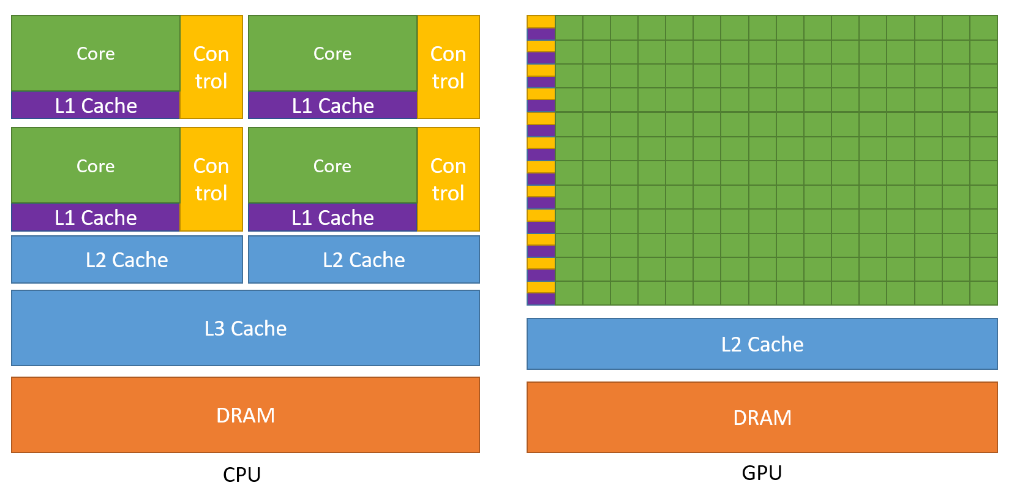
\includegraphics[width=\textwidth]{imagenes/chapter2/cpuvsgpu.PNG}
    \caption{Diferencia de arquitectura entre una CPU y una GPU. Extraído de~\cite{cuda-programming-guide}.}
    \label{fig:cpuvsgpu}
\end{figure}


Si se estudia la arquitectura de las GPUs, es necesario abordar también CUDA, %(sigla que abrevia Compute Unified Device Architecture)
%y su paralelismo o mapeo con las estructuras que este tipo de dispositivos (de la marca NVIDIA) ofrece.
término utilizado no solamente para describir la arquitectura de hardware presentada en 2006 por la compañía \texttt{NVIDIA}, sino también para referirse al modelo y lenguaje de programación que permite crear aplicaciones que ejecutan en estos dispositivos. 

Desde el punto de vista del modelo de programación, la ejecución del programa se distribuye en hilos (\textit{threads}), organizados en una grilla indexada llamada bloque (\textit{threadblock}), y a su vez, estos bloques también forman una grilla indexada (\textit{grid}). A priori, la ejecución de los hilos y bloques es totalmente independiente y puede darse en cualquier orden. El lenguaje de programación consiste en una extensión del lenguaje C, que permite, entre otras cosas, la creación de estas grillas de hilos, la programación de las funciones a ejecutar en el dispositivo (kernels) y las transferencias de datos entre la CPU y la GPU.

Por su parte, la arquitectura de hardware se forma entorno a una serie de multi-procesadores paralelos (Streaming Multiprocessors o SMs), cada uno formado por varios núcleos. La cantidad de procesadores y núcleos con los que cuenta la GPU varía según las diferentes generaciones de tarjetas. 
La memoria de las GPUs se organiza de forma jerárquica. En un primer nivel, existe una memoria global relativamente lenta pero accesible por todos los hilos. Se encuentra fuera de los multiprocesadores, por lo que el acceso a la misma implica una alta latencia, pero también posee un gran ancho de banda. Adicionalmente, a partir de la segunda generación de CUDA, se incluye una memoria caché de segundo nivel. Dentro de cada multiprocesador, existe una memoria de baja latencia pero de mucho menor tamaño con respecto a la global. Esta memoria es compartida físicamente por los bloques de hilos que residen en el multiprocesador. Por último, cada multiprocesador contiene un archivo de registros el cual es repartido entre todos los hilos residentes en el multiprocesador. Los registros son la memoria más rápida que brinda la GPU, pero también es la más reducida en tamaño.

Existe cierta correspondencia entre este modelo abstracto y la arquitectura de hardware. Siguiendo el espíritu de la clasificación de sistemas paralelos propuesta por Flynn en \cite{Flynn1972}, NVIDIA clasifica su arquitectura como Single Instruction Multiple Thread o SIMT. A diferencia de la categoría SIMD, en la cual una misma instrucción  se ejecuta simultáneamente sobre distintos elementos de un conjunto de datos, en SIMT el usuario puede  especificar distintos flujos de ejecución para los distintos hilos, aunque dadas las características  del hardware, el desempeño es mucho mayor cuando el comportamiento de la aplicación se asemeja al tipo SIMD.
 
Comenzada la ejecución del programa, cada multiprocesador se encarga de la ejecución concurrente de un grupo fijo de bloques, como se muestra en la Figura~\ref{fig:cuda-gpu}. Los hilos pertenecientes a estos bloques son divididos, planificados y ejecutados en grupos de 32 hilos llamados warps. La división se realiza siempre de forma que los hilos con índice 0 a 31 forman el primer warp, los de índice 32 a 63 al segundo, y así sucesivamente. La ejecución se organiza de forma que los threads de un mismo warp deben ejecutar la misma instrucción en cada momento. Dado el caso, si en el flujo de ejecución de distintos hilos del mismo warp, dos hilos divergen, debiendo ejecutar distintas instrucciones, las mismas se ejecutan de forma secuencial y los hilos que ejecutan una de las instrucciones quedan inactivos hasta que el resto de los hilos del warp ejecuten la otra instrucción. Por esta razón, la máxima eficiencia es alcanzada cuando todos los hilos de un warp ejecutan la misma instrucción en todo momento, aunque la misma se ejecute sobre distintos elementos del conjunto de datos. La asignación de recursos a cada warp dentro de un multiprocesador se realiza de forma estática, asignando un segmento del archivo de registros (\textit{register file}) a cada warp, y asignando una sección de la memoria compartida del multiprocesador a cada bloque que ejecuta en él. De esta forma, el cambio de contexto entre un warp y otro se realiza sin costo. 
Otro aspecto muy importante son los accesos a memoria. No sólo es una mejora importante que cada hilo de un mismo warp ejecute la misma instrucción, sino que es importante también que ejecuten utilizando datos que se encuentren en espacios de memoria contiguos, produciendo accesos \textit{coalesced}. El acceso a memoria \textit{coalesced}, refiere a combinar múltiples accesos a la memoria en una sola transacción. %Por ejemplo en las GPU K20, se puede acceder a 128 bytes contiguos (32 palabras en simple precisión) mediante un warp (32 hilos consecutivos) en una sola transacción. 


Junto con CUDA, NVIDIA provee un conjunto de herramientas que continúan en desarrollo gracias a los aportes de investigadores, las cuales tienen como objetivo complementar la arquitectura mejorando su usabilidad en distintas áreas de aplicación. Entre estas herramientas se encuentran lenguajes como \texttt{CUDA FORTRAN}, \texttt{PyCUDA}, APIs como \texttt{OpenACC} o \texttt{PGI Accelerator Compiler}, herramientas de análisis, debugging, y un gran conjunto de bibliotecas optimizadas en GPU, como por ejemplo \texttt{cuBLAS}~\cite{cublas} y \texttt{cuSPARSE}~\cite{cusparse}.


\begin{figure}
    \centering
    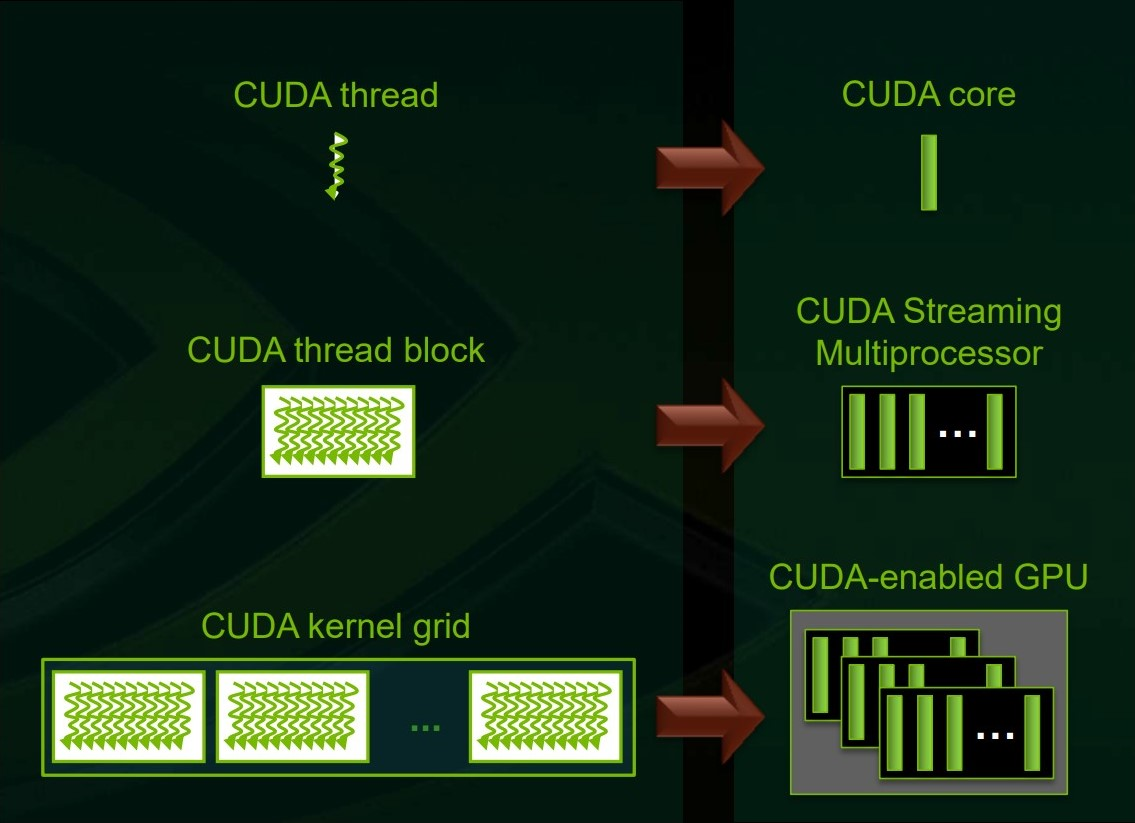
\includegraphics[width=0.7\textwidth]{imagenes/chapter2/cuda-gpu.jpg}
    \caption{Mapeo entre estructuras CUDA y GPU. Extraído de \cite{cuda-programming-guide}.}
    \label{fig:cuda-gpu}
\end{figure}


\subsection{Algoritmos en HPC}

En general, el cuello de botella de la mayoría de las operaciones y algoritmos que se ejecutan en arquitecturas de HPC al día de hoy, se da en los accesos a memoria, debido principalmente a la alta latencia de los mismos en relación a la de las %o ancho de banda significativamente más lento que estas presentan con respecto a la cantidad de 
operaciones aritméticas (operaciones en punto flotante FLOPS). Muchos cálculos científicos sólo aprovechan una fracción de la potencia computacional en las arquitecturas de alto rendimiento actuales. La dificultad radica, en muchos casos, en mapear dichas operaciones a las arquitecturas, intentando explotar al máximo los atributos de cómputo que presentan haciendo uso de, por ejemplo, jerarquías de memoria con el objetivo de mitigar la baja latencia de las memorias principales.

Al mismo tiempo, las operaciones de memoria son el principal consumidor de energía de las arquitecturas modernas, lo que afecta en gran medida el costo de los recursos, como se puede observar en la Figura~\ref{fig:horowitz-energy}. Un estudio  detallado de este y otros problemas es el que plantea Horowitz en~\cite{Horowitz2014}.

\begin{figure}
    \centering
    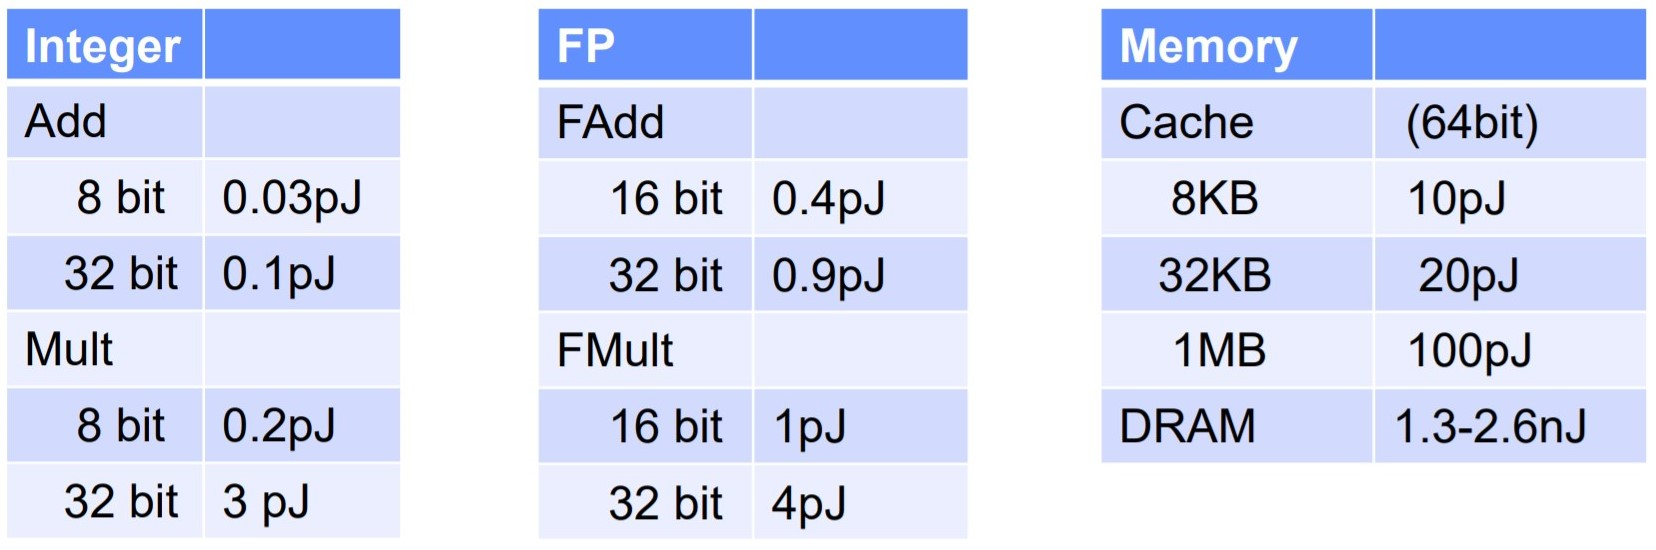
\includegraphics[width=\textwidth]{imagenes/chapter2/horowitz-energy.jpg}
    \caption{Valores aproximados de energía consumida por operación (45nm). Extraído de~\cite{Horowitz2014}.}
    \label{fig:horowitz-energy}
\end{figure}

El ALN no escapa de este paradigma, en particular, las operaciones con matrices dispersas encajan perfectamente en esta categoría de problemas. Entre los varios problemas del ALN dispersa, la SpMV es un claro ejemplo de operación con un costo computacional razonable a nivel de operaciones, y que puede ser atacada de forma paralela, pero que se ve fuertemente limitada por el ancho de banda entre procesador y memoria, 
además su baja intensidad computacional, es decir, la baja cantidad de operaciones aritméticas realizadas por cada acceso a memoria, sumada a la aleatoriedad de los accesos que implica un pobre aprovechamiento de los caches, produciendo un ratio bajo de lecturas efectivas.

En este contexto, es de gran interés estudiar formatos ``óptimos'' para matrices dispersas, que logren reducir la cantidad de transacciones de memoria o, al menos, ofrezcan mejoras mediante el acceso de forma ordenada, aprovechando así en lo posible el ancho de banda limitado.





